\begin{frame}{Problemas Relajados continuación}
Ejemplo bien conocido: \emphblue{problema del vendedor ambulante} (TSP)
Encuentra el recorrido más corto visitando todas las ciudades exactamente una vez\\
\begin{center}
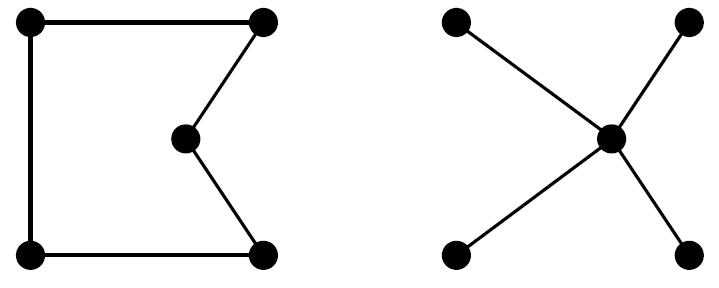
\includegraphics[scale=0.4]{35_image_mst.PNG}\\
\end{center}

\emphblue{El árbol de expansión mínimo} se puede calcular en \textcolor{magenta}{$O (n2)$} 
y es un límite inferior en el recorrido más corto (abierto)

\end{frame}